\documentclass{ltxdoc}
\title{Commutative LBC Actions Proposal}

\usepackage{amsmath}  % extended mathematics
\usepackage{units}    % non-stacked fractions and better unit spacing
\usepackage{fancyvrb} % extended verbatim environments
\usepackage{tikz}
\usepackage{printlen}
\usepackage{tkz-berge}
\usepackage{mathtools}
\usepackage{forest}
\usepackage{xcolor}
\usepackage[margin=0.5in]{geometry}
\usetikzlibrary{arrows,arrows.meta,chains, decorations.pathreplacing, shapes.multipart}

\begin{document}

%\forestset{
  %default preamble={
    %for tree={circle,draw}
  %}
%}

\section{Playground}

\vspace{30px}

\definecolor{syellow}{RGB}{181,137,0}
\definecolor{sorange}{RGB}{203,75,22}
\definecolor{sred}{RGB}{220,50,47}
\definecolor{smagenta}{RGB}{211,54,130}
\definecolor{sviolet}{RGB}{108,113,196}
\definecolor{sblue}{RGB}{38,139,210}
\definecolor{scyan}{RGB}{42,161,152}
\definecolor{sgreen}{RGB}{133,153,0}

\newcommand\measurexdistance[5][####1]{\measurexorydistance{#2}{#3}{#4}{#5}{\x}{-|}{(5pt,0)}{#1}}
\newcommand\measureydistance[5][####1]{\measurexorydistance{#2}{#3}{#4}{#5}{\y}{|-}{(0,5pt)}{#1}}
\tikzset{dimension/.style={<->,>=latex,thin,every rectangle node/.style={midway,font=\scriptsize}},
 guideline/.style=dotted}
\newdimen\absmd
\def\measurexorydistance#1#2#3#4#5#6#7#8{%
 \path #1 #3 #6 coordinate(md1) #1; \draw[guideline] #1 -- (md1);
 \path (md1) #6 coordinate(md2) #2; \draw[guideline] #2 -- (md2);
 \path let \p1=($(md1)-(md2)$), \n1={abs(#51)} in \pgfextra{\xdef\md{#51}\global\absmd=\n1\relax};
 \def\distancelabelwrapper##1{#8}%
 \ifdim\absmd>5mm
 \draw[dimension] (md1)--(md2) node[#4]{\distancelabelwrapper{\uselengthunit{mm}\rndprintlength\absmd}};
 \else
 \ifdim\md>0pt
 \draw[dimension,<-] (md1)--+#7; \draw[dimension,<-] let \p1=($(0,0)-#7$) in (md2)--+(\p1);
 \else
 \draw[dimension,<-] let \p1=($(0,0)-#7$) in (md1)--+(\p1); \draw[dimension,<-] (md2)--+#7;
 \fi
 \draw[dimension,-] (md1)--(md2) node[#4]{\distancelabelwrapper{\uselengthunit{mm}\rndprintlength\absmd}};
 \fi}

\begin{forest}
  for tree={grow=east,s sep=8pt,l=0.5pt,inner sep=2pt}
  [,circle,draw,name=oldest
    [,circle,draw,edge=dotted
    [,circle,draw,edge=dotted
    [,circle,draw,edge=dotted
    [,circle,draw,edge=dotted
    [,circle,draw,edge=dotted
    [,circle,draw,edge=dotted,name=locked
    [,circle,draw
      [,circle,draw
            [,circle,draw
              [,circle,draw
                [,circle,draw
                  [,circle,draw]]]
              [,circle,draw
                [,circle,draw
                  [,circle,draw
                    [,circle,draw,name=best]]]]
              [,circle,draw]]
            [,circle,draw]]]
    ]]]]]]]
    \measurexdistance[$k=2160$]
 {(locked.north)}{(best.north)}{(.north)+(0,6mm)}{above}
    \measurexdistance[$k=2160$]
 {(oldest.north)}{(locked.south)}{(.south)+(0,-3mm)}{below}
\end{forest}

\vspace{30px}

\begin{forest}
  for tree={grow=east,s sep=8pt,l=0.5pt,inner sep=2pt}
    [,circle,draw,for tree={edge={Latex-}}
      [,circle,draw
            [,circle,draw
              [,circle,draw
                [,circle,draw
                  [,circle,draw]]]
              [,circle,draw
                [,circle,draw
                  [,circle,draw
                    [,circle,draw,name=best]]]]
              [,circle,draw]]
            [,circle,draw]]]
\end{forest}




\vspace{30px}

\section{Concrete}

\vspace{30px}

\[ \sigma_0 T_0^1 \sigma_1 \]

\vspace{30px}

\[ \Sigma \]

\vspace{30px}

\[ \sigma_0 \]

\vspace{30px}

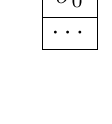
\begin{tikzpicture}[
   double/.style={draw, anchor=text, rectangle split,rectangle split parts=2}
  ]
      \tikz{\node[double]{$\sigma_0$ \nodepart{second} $\cdots$ }}

\end{tikzpicture}

\vspace{30px}

\[ \Sigma_0 \]

\vspace{30px}

\[ \Rightarrow \! \! \Sigma_0 \]

\vspace{30px}

\[ \sigma_0 \implies \sigma_1 \]

\vspace{30px}

\begin{align*}
  \sigma_0 + T_0^1 &= \sigma_1 \\
  \sigma_1 + T_1^2 &= \sigma_2 \\
  \sigma_2 + T_2^3 &= \sigma_3
\end{align*}

\vspace{30px}

\begin{forest}
% TODO: Draw the rectangles
  [$\sigma_0$,
    [$T_0^1$ [$\sigma_1$ [$T_1^2$ [$\sigma_2$]]]]]
\end{forest}

\vspace{30px}

\begin{forest}
    [,circle,draw,tier=top,name=b1,fit=rectangle
     [$\sigma_0 \implies \sigma_4$,edge=dashed
       [$\sigma_0 \implies \sigma_2$
         [$\sigma_0 \implies \sigma_1$ [$\sigma_0 \; T_0^1 \; \sigma_1$,magenta ] ]
         [$\sigma_1 \implies \sigma_2$ [$\sigma_1 \; T_1^2 \; \sigma_2$,magenta ] ]
       ]
       [$\sigma_2 \implies \sigma_4$
         [$\sigma_2 \implies \sigma_3$ [$\sigma_2 \; T_2^3 \; \sigma_3$,magenta ] ]
         [$\sigma_3 \implies \sigma_4$ [$\sigma_3 \; T_3^4 \; \sigma_4$,magenta ] ]
       ]
     ]
    ]
\end{forest}

\vspace{30px}

\section{Merging}

\vspace{30px}

A

\vspace{30px}

\begin{forest}
[$\sigma_0 \implies \sigma_2$
   [$\sigma_0 \implies \sigma_1$]
   [$\sigma_1 \implies \sigma_2$]
]
\end{forest}

\vspace{30px}

B (left/right paren)

\vspace{30px}

\begin{forest}
  [,phantom
    [$\sigma_0 \implies \sigma_3$,name=left,for tree={green!50!black}
      [$\sigma_0 \implies \sigma_2$
       [$\sigma_0 \implies \sigma_1$]
       [$\sigma_1 \implies \sigma_2$]
      ]
      [$\sigma_2 \implies \sigma_3$]
    ]
    [$\sigma_0 \implies \sigma_3$,name=right,for tree={purple!80!black}
      [$\sigma_0 \implies \sigma_1$]
      [$\sigma_1 \implies \sigma_3$
       [$\sigma_1 \implies \sigma_2$]
       [$\sigma_2 \implies \sigma_3$]
      ]
    ]
  ]
  \draw[dotted,<->] (left) to[out=east,in=west] (right);
\end{forest}

\vspace{30px}

\section{Serial}

\vspace{30px}

\begin{forest}
  [,phantom,name=b0,fit=rectangle,s sep=1.5em
    [$\sigma_0 \implies \sigma_0$,tier=mid,name=i00]
      [,circle,draw,tier=top,name=s01,fit=rectangle
        [$\sigma_0 \implies \sigma_1$,tier=mid,edge={dashed,<-},name=i01 [$\sigma_0 \; T_0^1 \; \sigma_1$,magenta,edge={<-}] ]
      ]
      [,circle,draw,tier=top,name=s02,fit=rectangle
        [$\sigma_0 \implies \sigma_2$,tier=mid,edge={dashed,<-},name=i02 [$\sigma_1 \; T_1^2 \; \sigma_2$,magenta,edge={<-},name=i12] ]
      ]
      [,circle,draw,tier=top,name=s03,fit=rectangle
        [$\sigma_0 \implies \sigma_3$,tier=mid,edge={dashed,<-},name=i03 [$\sigma_2 \; T_2^3 \; \sigma_3$,magenta,edge={<-},name=i23] ]
      ]
      [,circle,draw,tier=top,name=s04,fit=rectangle
        [$\sigma_0 \implies \sigma_4$,tier=mid,edge={dashed,<-},name=i04 [$\sigma_3 \; T_3^4 \; \sigma_4$,magenta,edge={<-},name=i34] ]
      ]
  ]
  %\draw[->] (b0) to[out=south,in=west] (s01);
  %\draw[->] (s01) to[out=east,in=west] (s02);
  %\draw[->] (s02) to[out=east,in=west] (s03);
  %\draw[->] (s03) to[out=east,in=north] (b1);
  \draw[->] (i00) to[out=east,in=south] (i01);
  \draw[->] (i01) to[out=east,in=south] (i02);
  \draw[->] (i02) to[out=east,in=south] (i03);
  \draw[->] (i03) to[out=east,in=south] (i04);
\end{forest}


\vspace{30px}

\section{Pre-naive}

\vspace{30px}

\[ A_0^1 \coloneqq \; \; \sigma_0 T_0^1 \sigma_1 \]

\vspace{30px}

\[ B_0^2 \coloneqq \; \; \sigma_0 \implies \sigma_2 \]

\vspace{30px}

\[ ((((A + A_1) + A_2) + A_3) + A_4) \]

\vspace{30px}

\section{Naive}

\vspace{30px}

Data

\vspace{30px}

\begin{forest}
 [,phantom
   [,phantom
     [,phantom
       [,phantom [$A_0^1$] ]
       [,phantom [$A_1^2$] ]
     ]
     [,phantom
       [,phantom [$A_2^3$] ]
       [,phantom [$A_3^4$] ]
     ]
   ]
   [,phantom
     [,phantom
       [,phantom [$A_4^5$] ]
       [,phantom [$A_5^6$] ]
     ]
     [,phantom
       [,phantom [$A_6^7$] ]
       [,phantom [$A_7^8$] ]
     ]
   ]
 ]
\end{forest}

\vspace{30px}

Base proofs

\vspace{30px}

\begin{forest}
 [,phantom
   [,phantom
     [,phantom
       [$B_0^1$ [$A_0^1$] ]
       [$B_1^2$ [$A_1^2$] ]
     ]
     [,phantom
       [$B_2^3$ [$A_2^3$] ]
       [$B_3^4$ [$A_3^4$] ]
     ]
   ]
   [,phantom
     [,phantom
       [$B_4^5$ [$A_4^5$] ]
       [$B_5^6$ [$A_5^6$] ]
     ]
     [,phantom
       [$B_6^7$ [$A_6^7$] ]
       [$B_7^8$ [$A_7^8$] ]
     ]
   ]
 ]
\end{forest}

\vspace{30px}

Merge proofs

\vspace{30px}

\begin{forest}
 [,phantom
   [,phantom
     [$B_0^2$
       [$B_0^1$ [$A_0^1$] ]
       [$B_1^2$ [$A_1^2$] ]
     ]
     [$B_2^4$
       [$B_2^3$ [$A_2^3$] ]
       [$B_3^4$ [$A_3^4$] ]
     ]
   ]
   [,phantom
     [$B_4^6$
       [$B_4^5$ [$A_4^5$] ]
       [$B_5^6$ [$A_5^6$] ]
     ]
     [$B_6^8$
       [$B_6^7$ [$A_6^7$] ]
       [$B_7^8$ [$A_7^8$] ]
     ]
   ]
 ]
\end{forest}

\vspace{30px}

All the way

\vspace{30px}

\begin{forest}
 [,phantom
   [$B_0^4$
     [$B_0^2$
       [$B_0^1$ [$A_0^1$] ]
       [$B_1^2$ [$A_1^2$] ]
     ]
     [$B_2^4$
       [$B_2^3$ [$A_2^3$] ]
       [$B_3^4$ [$A_3^4$] ]
     ]
   ]
   [$B_4^8$
     [$B_4^6$
       [$B_4^5$ [$A_4^5$] ]
       [$B_5^6$ [$A_5^6$] ]
     ]
     [$B_6^8$
       [$B_6^7$ [$A_6^7$] ]
       [$B_7^8$ [$A_7^8$] ]
     ]
   ]
 ]
\end{forest}

\vspace{30px}

\begin{forest}
  [,phantom
    [$B_0^0$,tier=top,name=b0,calign=first]
    [$B_0^8$,tier=top,name=b1,fit=rectangle
     [$B_0^8$,edge=dotted
       [$B_0^4$
         [$B_0^2$
           [$B_0^1$ [$A_0^1$] ]
           [$B_1^2$ [$A_1^2$] ]
         ]
         [$B_2^4$
           [$B_2^3$ [$A_2^3$] ]
           [$B_3^4$ [$A_3^4$] ]
         ]
       ]
       [$B_4^8$
         [$B_4^6$
           [$B_4^5$ [$A_4^5$] ]
           [$B_5^6$ [$A_5^6$] ]
         ]
         [$B_6^8$
           [$B_6^7$ [$A_6^7$] ]
           [$B_7^8$ [$A_7^8$] ]
         ]
       ]
     ]
    ]
  ]
\end{forest}

\vspace{30px}

\section{Better Solution}

\vspace{30px}

I wish we could lay horizontal?

A

\vspace{30px}

\begin{forest}
   [,phantom
     [,phantom, for tree={scyan}
       [,phantom
         [,phantom [$A_0^1$] ]
         [,phantom [$A_1^2$] ]
       ]
       [,phantom
         [,phantom [$A_2^3$] ]
         [,phantom [$A_3^4$] ]
       ]
     ]
     [,phantom, for tree={sviolet}
       [,phantom
         [,phantom [,phantom ] ] ]
       [,phantom 
         [,phantom [,phantom ] ] ]
     ]
   ]
\end{forest}

\vspace{30px}

A.5

\vspace{30px}

\begin{forest}
   [,phantom
     [,phantom, for tree={scyan}
       [,phantom
         [$B_0^1$ [$A_0^1$] ]
         [$B_1^2$ [$A_1^2$] ]
       ]
       [,phantom
         [$B_2^3$ [$A_2^3$] ]
         [$B_3^4$ [$A_3^4$] ]
       ]
     ]
     [,phantom, for tree={sviolet}
       [,phantom
         [,phantom [$A_4^5$] ]
         [,phantom [$A_5^6$] ]
       ]
       [,phantom
         [,phantom [$A_6^7$] ]
         [,phantom [$A_7^8$] ]
       ]
     ]
   ]
\end{forest}

\vspace{30px}

A.5

\vspace{30px}

\begin{forest}
   [,phantom
     [,phantom, for tree={scyan}
       [$B_0^2$
         [$B_0^1$ [$A_0^1$] ]
         [$B_1^2$ [$A_1^2$] ]
       ]
       [$B_2^4$
         [$B_2^3$ [$A_2^3$] ]
         [$B_3^4$ [$A_3^4$] ]
       ]
     ]
     [,phantom, for tree={sviolet}
       [,phantom
         [$B_4^5$ [$A_4^5$] ]
         [$B_5^6$ [$A_5^6$] ]
       ]
       [,phantom
         [$B_6^7$ [$A_6^7$] ]
         [$B_7^8$ [$A_7^8$] ]
       ]
     ]
     [,phantom, for tree={sorange}
       [,phantom
         [,phantom [$A_8^9$] ]
         [,phantom [$A_9^{10}$] ]
       ]
       [,phantom
         [,phantom [$A_{10}^{11}$] ]
         [,phantom [$A_{11}^{12}$] ]
       ]
     ]
   ]
\end{forest}

\vspace{30px}

A.5

\vspace{30px}

\begin{forest}
  [,phantom
   [$B_0^0$,tier=top,name=b0,calign=first]
   [$B_0^4$,tier=top,name=b1,fit=rectangle
     [$B_0^4$,edge=dotted, for tree={scyan}
       [$B_0^2$
         [$B_0^1$ [$A_0^1$] ]
         [$B_1^2$ [$A_1^2$] ]
       ]
       [$B_2^4$
         [$B_2^3$ [$A_2^3$] ]
         [$B_3^4$ [$A_3^4$] ]
       ]
     ]
   ]
   [,phantom,tier=top
     [,phantom, for tree={sviolet}
       [$B_4^6$
         [$B_4^5$ [$A_4^5$] ]
         [$B_5^6$ [$A_5^6$] ]
       ]
       [$B_6^8$
         [$B_6^7$ [$A_6^7$] ]
         [$B_7^8$ [$A_7^8$] ]
       ]
     ]
   ]
   [,phantom,tier=top
     [,phantom, for tree={sorange}
       [,phantom
         [$B_8^9$ [$A_8^9$] ]
         [$B_9^{10}$ [$A_9^{10}$] ]
       ]
       [,phantom
         [$B_{10}^{11}$ [$A_{10}^{11}$] ]
         [$B_{11}^{12}$ [$A_{11}^{12}$] ]
       ]
     ]
   ]
   [,phantom,tier=top
     [,phantom, for tree={scyan}
       [,phantom
         [,phantom [$A_{12}^{13}$] ]
         [,phantom [$A_{13}^{14}$] ]
       ]
       [,phantom
         [,phantom [$A_{14}^{15}$] ]
         [,phantom [$A_{15}^{16}$] ]
       ]
     ]
   ]
   ]
\end{forest}

\vspace{30px}

B

\vspace{30px}

\begin{forest}
  [,phantom
   [$B_0^0$,tier=top,name=b0,calign=first]
   [$B_0^4$,tier=top,name=b1,fit=rectangle
     [$B_0^4$,edge=dotted, for tree={scyan}
       [$B_0^2$
         [$B_0^1$ [$A_0^1$] ]
         [$B_1^2$ [$A_1^2$] ]
       ]
       [$B_2^4$
         [$B_2^3$ [$A_2^3$] ]
         [$B_3^4$ [$A_3^4$] ]
       ]
     ]
   ]
   [$B_4^8$,tier=top
     [$B_4^8$, for tree={sviolet}
       [$B_4^6$
         [$B_4^5$ [$A_4^5$] ]
         [$B_5^6$ [$A_5^6$] ]
       ]
       [$B_6^8$
         [$B_6^7$ [$A_6^7$] ]
         [$B_7^8$ [$A_7^8$] ]
       ]
     ]
   ]
   [,phantom,tier=top
     [,phantom, for tree={sorange}
       [$B_8^{10}$
         [$B_8^9$ [$A_8^9$] ]
         [$B_9^{10}$ [$A_9^{10}$] ]
       ]
       [$B_{10}^{12}$
         [$B_{10}^{11}$ [$A_{10}^{11}$] ]
         [$B_{11}^{12}$ [$A_{11}^{12}$] ]
       ]
     ]
   ]
   [,phantom,tier=top
     [,phantom, for tree={scyan}
       [,phantom
         [$B_{12}^{13}$ [$A_{12}^{13}$] ]
         [$B_{13}^{14}$ [$A_{13}^{14}$] ]
       ]
       [,phantom
         [$B_{14}^{15}$ [$A_{14}^{15}$] ]
         [$B_{15}^{16}$ [$A_{15}^{16}$] ]
       ]
     ]
   ]
   ]
\end{forest}

\vspace{30px}

C

\vspace{30px}

\begin{forest}
  [,phantom
   [$B_0^4$,tier=top,name=b0,calign=first]
   [$B_4^8$,tier=top,name=b1,fit=rectangle
     [$B_4^8$, for tree={sviolet}
       [$B_4^6$
         [$B_4^5$ [$A_4^5$] ]
         [$B_5^6$ [$A_5^6$] ]
       ]
       [$B_6^8$
         [$B_6^7$ [$A_6^7$] ]
         [$B_7^8$ [$A_7^8$] ]
       ]
     ]
     ]
   [$B_8^{12}$,tier=top
     [$B_8^{12}$, for tree={sorange}
       [$B_8^{10}$
         [$B_8^9$ [$A_8^9$] ]
         [$B_9^{10}$ [$A_9^{10}$] ]
       ]
       [$B_{10}^{12}$
         [$B_{10}^{11}$ [$A_{10}^{11}$] ]
         [$B_{11}^{12}$ [$A_{11}^{12}$] ]
       ]
     ]
   ]
   [,phantom,tier=top
     [,phantom, for tree={scyan}
       [$B_{12}^{14}$
         [$B_{12}^{13}$ [$A_{12}^{13}$] ]
         [$B_{13}^{14}$ [$A_{13}^{14}$] ]
       ]
       [$B_{14}^{16}$
         [$B_{14}^{15}$ [$A_{14}^{15}$] ]
         [$B_{15}^{16}$ [$A_{15}^{16}$] ]
       ]
     ]
   ]
   [,phantom,tier=top
     [,phantom, for tree={sviolet}
       [,phantom
         [$B_{16}^{17}$ [$A_{16}^{17}$] ]
         [$B_{17}^{18}$ [$A_{17}^{18}$] ]
       ]
       [,phantom
         [$B_{18}^{19}$ [$A_{18}^{19}$] ]
         [$B_{19}^{20}$ [$A_{19}^{20}$] ]
       ]
     ]
   ]
   ]
\end{forest}

\vspace{30px}

\section{Space Waste}

\vspace{30px}

\begin{forest}
  [,phantom
   [$B_0^0$,tier=top,name=b0,calign=first]
   [$B_0^4$,tier=top,name=b1,fit=rectangle
     [$B_0^4$,edge=dotted, for descendants={sred}
       [$B_0^2$
         [$B_0^1$ [$A_0^1$] ]
         [$B_1^2$ [$A_1^2$] ]
       ]
       [$B_2^4$
         [$B_2^3$ [$A_2^3$] ]
         [$B_3^4$ [$A_3^4$] ]
       ]
     ]
   ]
   [,phantom,tier=top
     [,phantom
       [$B_4^6$, for descendants={sred}
         [$B_4^5$ [$A_4^5$] ]
         [$B_5^6$ [$A_5^6$] ]
       ]
       [$B_6^8$, for descendants={sred}
         [$B_6^7$ [$A_6^7$] ]
         [$B_7^8$ [$A_7^8$] ]
       ]
     ]
   ]
   [,phantom,tier=top
     [,phantom
       [,phantom
         [$B_8^9$, for descendants={sred} [$A_8^9$] ]
         [$B_9^{10}$, for descendants={sred} [$A_9^{10}$] ]
       ]
       [,phantom
         [$B_{10}^{11}$, for descendants={sred} [$A_{10}^{11}$] ]
         [$B_{11}^{12}$, for descendants={sred} [$A_{11}^{12}$] ]
       ]
     ]
   ]
   [,phantom,tier=top
     [,phantom
       [,phantom
         [,phantom [$A_{12}^{13}$] ]
         [,phantom [$A_{13}^{14}$] ]
       ]
       [,phantom
         [,phantom [$A_{14}^{15}$] ]
         [,phantom [$A_{15}^{16}$] ]
       ]
     ]
   ]
   ]
\end{forest}

\vspace{30px}

Compress it

\vspace{30px}

\begin{forest}

  [,phantom
   [$B_0^0$,tier=top,name=b0,calign=first]
   [$B_0^4$,tier=top,name=b1,fit=rectangle,scyan
     [$B_0^4$,edge=dotted,scyan
       [$B_4^6$,sviolet
         [$B_8^9$,sorange [$A_{12}^{13}$,scyan] ]
         [$B_9^{10}$,sorange [$A_{13}^{14}$,scyan] ]
       ]
       [$B_6^8$,sviolet
         [$B_{10}^{11}$,sorange [$A_{14}^{15}$,scyan] ]
         [$B_{11}^{12}$,sorange [$A_{15}^{16}$,scyan] ]
       ]
     ]
   ]
  ]
\end{forest}

Part 2

\begin{forest}
  [,phantom
   [$B_0^4$,tier=top,name=b0,calign=first,scyan]
   [$B_4^8$,tier=top,name=b1,fit=rectangle,sviolet
     [$B_4^8$,edge=dotted,sviolet
       [$B_8^{10}$,sorange
         [$B_{12}^{13}$,scyan [$A_{16}^{17}$,sviolet] ]
         [$B_{13}^{14}$,scyan [$A_{17}^{18}$,sviolet] ]
       ]
       [$B_{10}^{12}$,sorange
         [$B_{14}^{15}$,scyan [$A_{18}^{19}$,sviolet] ]
         [$B_{15}^{16}$,scyan [$A_{19}^{20}$,sviolet] ]
       ]
     ]
   ]
  ]
\end{forest}

\section{Instantiation}

\vspace{30px}

\begin{forest}
  [,phantom
    [$\Rightarrow \! \! \Sigma_0$,tier=top,name=b0,calign=first]
    [$\Rightarrow \! \! \Sigma_1$,tier=top,name=b1,fit=rectangle
     [$\sigma_0 \implies \sigma_4$,edge=dotted
       [$\sigma_4 \implies \sigma_6$
         [,circle,draw [$\sigma_8 \; T_8^9 \; \sigma_9$,magenta] ]
         [,circle,draw [$\sigma_9 \; T_9^{10} \; \sigma_{10}$,magenta] ]
       ]
       [,circle,draw
         [$\sigma_6 \implies \sigma_7$ [,circle,draw] ]
         [$\sigma_7 \implies \sigma_8$ [,circle,draw] ]
       ]
     ]
    ]
  ]
  \draw[->] (b0) to[out=east,in=west] (b1);
\end{forest}

\vspace{30px}

\begin{forest}
  [$B(B_{12}^{14}; B_{14}^{16})$
     [$B(B_{16}^{17}; B_{17}^{18})$
       [$B(A_{20}^{21})$ ]
       [$B(A_{21}^{22})$ ]
     ]
     [$B(B_{18}^{19}; B_{19}^{20})$
       [$B(A_{22}^{23})$ ]
       [$B(A_{23}^{24})$ ]
     ]
   ]
\end{forest}

\vspace{30px}

\section{Succinct}

\vspace{30px}

% https://tex.stackexchange.com/questions/245251/proportional-boxes-in-tikz-array-diagram
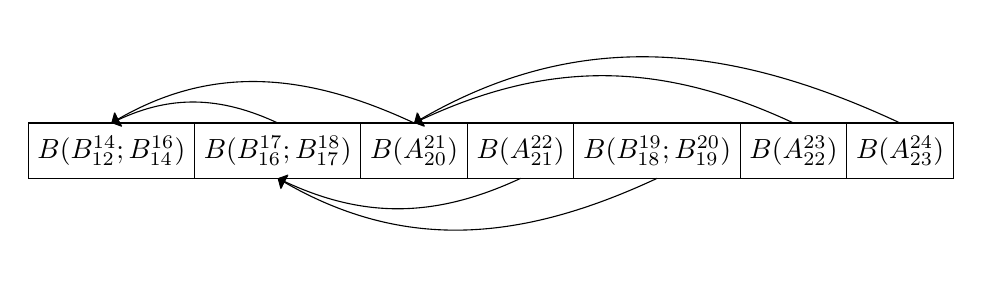
\begin{tikzpicture}[
%  -{Stealth[length = 2.5pt]},
       start chain = going right,
     node distance = 0pt,
MyStyle/.style={draw, minimum width=2em, minimum height=2em, 
                outer sep=0pt, on chain},
  ]
\node [MyStyle] (1) {$B(B_{12}^{14}; B_{14}^{16})$};
  \node [MyStyle] (2) {$B(B_{16}^{17}; B_{17}^{18})$};
  \node [MyStyle] (3) {$B(A_{20}^{21})$};
  \node [MyStyle] (4) {$B(A_{21}^{22})$};
  \node [MyStyle] (5) {$B(B_{18}^{19}; B_{19}^{20})$};
  \node [MyStyle] (6) {$B(A_{22}^{23})$};
  \node [MyStyle] (7) {$B(A_{23}^{24})$};
\begin{scope}[-{Stealth[length = 2.5pt]}]
  \draw[arrows={-Triangle[angle=90:4pt]}] (2.north) [out=155, in=25] to (1.north);
  \draw[arrows={-Triangle[angle=90:4pt]}] (3.north) [out=155, in=30] to (1.north);
  \draw[arrows={-Triangle[angle=90:4pt]}] (4.south) [out=-155, in=-25] to (2.south);
  \draw[arrows={-Triangle[angle=90:4pt]}] (5.south) [out=-155, in=-30] to (2.south);
  \draw[arrows={-Triangle[angle=90:4pt]}] (6.north) [out=155, in=25] to (3.north);
  \draw[arrows={-Triangle[angle=90:4pt]}] (7.north) [out=155, in=30] to (3.north);
\end{scope}
%\draw[decorate,decoration={brace, amplitude=10pt, raise=5pt, mirror}]
%  (2.south west) to node[black,midway,below= 15pt] {$k$-elements} (7.south east);
\end{tikzpicture}


\end{document}
